\documentclass{article}
\usepackage[utf8]{inputenc}

\title{EEC-201 Final Project}
\author{Igor Sheremet and Jonathan Tivald }
\date{March 2021}

\usepackage{natbib}
\usepackage{graphicx}
\usepackage{listings}
\usepackage{xcolor}
\usepackage{float}
%\usepackage{enumitem}

\definecolor{codegreen}{rgb}{0,0.6,0}
\definecolor{codegray}{rgb}{0.5,0.5,0.5}
\definecolor{codepurple}{rgb}{0.58,0,0.82}
\definecolor{backcolour}{rgb}{0.95,0.95,0.92}

\lstdefinestyle{mystyle}{
    backgroundcolor=\color{backcolour},   
    commentstyle=\color{codegreen},
    keywordstyle=\color{magenta},
    numberstyle=\tiny\color{codegray},
    stringstyle=\color{codepurple},
    basicstyle=\ttfamily\footnotesize,
    breakatwhitespace=false,         
    breaklines=true,                 
    captionpos=b,                    
    keepspaces=true,                 
    numbers=left,                    
    numbersep=5pt,                  
    showspaces=false,                
    showstringspaces=false,
    showtabs=false,                  
    tabsize=2
}

\lstset{style=mystyle}

\begin{document}

\maketitle

\section{Problem 1}

\begin{figure}[H]
\centering
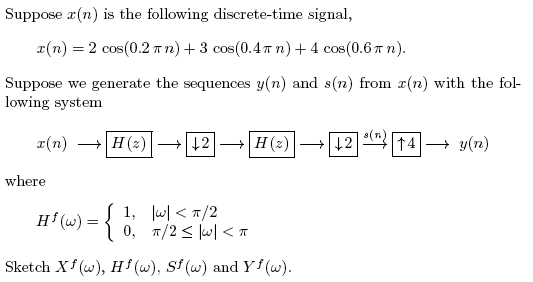
\includegraphics[scale=0.7]{Q1.png}
\end{figure}

\begin{lstlisting}[language=Matlab]
%%%%%%%%%%%%%%%%%%%%%%%%%%%%%%%%%%%%%%%
%Problem 1
%%%%%%%%%%%%%%%%%%%%%%%%%%%%%%%%%%%%%%%

%Parameters
wc = pi/2;
fs = 80;
sample_dur = 10;

%Generate "continuous" and "sampled" time stamps
tn = 0:1/fs:(sample_dur-(1/fs));
tnl = length(tn);

%Generate x[n]
xn = 2*cos(0.2*pi*tn)+3*cos(0.4*pi*tn)+4*cos(0.6*pi*tn);

%Generate s[n]
[xn_filt1,d] = lowpass(xn,wc,fs,'ImpulseResponse','iir','Steepness',0.99);
[hlp,flp] = freqz (d ,1024 , tnl ) ;
xn_dwn1 = downsample(xn_filt1,2);
xn_filt2 = lowpass(xn_dwn1,wc,fs/2,'ImpulseResponse','iir','Steepness',0.99);
sn = downsample(xn_filt2,2);

%Generate y[n]
yn = upsample(sn,4);

figure('name','Problem 1')

%Plot x[n]
subplot(4,2,1);
plot(tn,xn)
title('x[n]')

subplot(4,2,2);
N = tnl;
xk = fft(xn,N);
fk = (0:fs/N:fs-(fs/N));
plot(fk,abs(xk))
title('X[k]')

%Plot h[n]
subplot(4,2,3);
stem(0:1:length(d.Coefficients)-1, d.Coefficients(1,:))
hold on;
stem(0:1:length(d.Coefficients)-1, d.Coefficients(2,:),'r')
legend('b[n]','a[n]')
title('h[n]')

subplot(4,2,4);
plot(flp,mag2db(abs(hlp)))
title('H[k]')

%Plot s[n]
subplot(4,2,5);
plot(tn(1:4:end),sn)
title('s[n]')

subplot(4,2,6);
N = tnl/4;
sk = fft(sn,N);
fk = (0:fs/N:fs-(fs/N));
plot(fk,abs(sk))
title('S[k]')

%Plot y[n]
subplot(4,2,7);
stem(tn,yn)
title('y[n]')

subplot(4,2,8);
N = tnl;
yk = fft(yn,N);
fk = (0:fs/N:fs-(fs/N));
plot(fk,abs(yk))
title('Y[k]')
\end{lstlisting}

\begin{figure}[H]
\centering
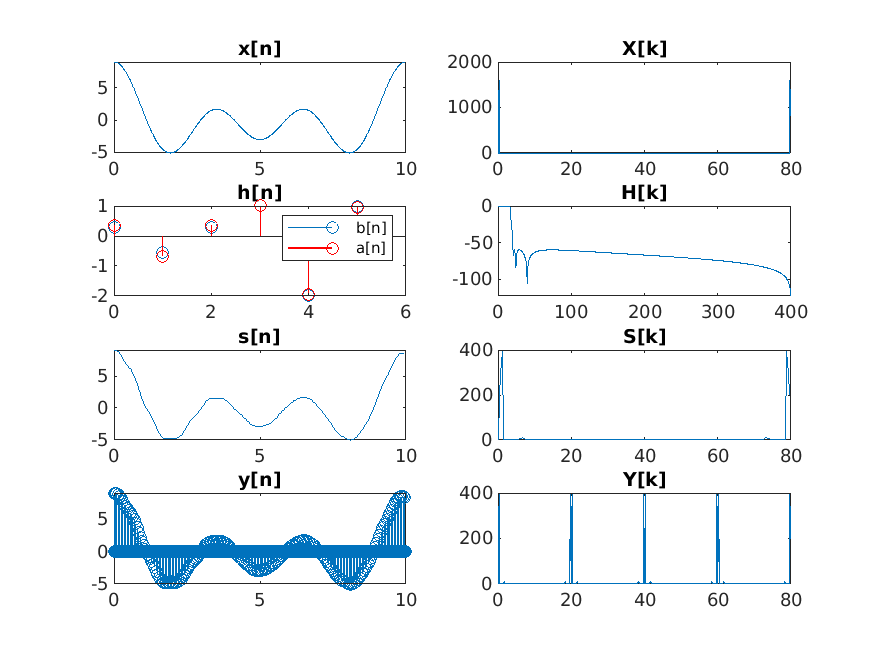
\includegraphics[scale=0.9]{problem1.png}
\end{figure}

\section{Problem 2}

\end{document}
